\section{Introduction}
\begin{multicols}{2}
En informatique, les Control Flow Graphs sont définis ainsi:
\begin{quotation}
    Un graphe de flot de contrôle (abrégé en GFC, control flow graph ou CFG en anglais) est une représentation sous forme de graphe de tous les chemins qui peuvent être suivis par un programme durant son exécution. \cite{wiki:Graphe_de_flot_de_controle}
\end{quotation}
A droite un exemple de CFG généré à partir du programme suivant:
\begin{lstlisting}
    int main() {
        int a = 0;
        
        while(a < 1000) {
            if(a % 2 == 0) {
                a++;
            }
            else {
                a+=2;
            }
        }
    
        return 0;
    }
\end{lstlisting}
\begin{center}
    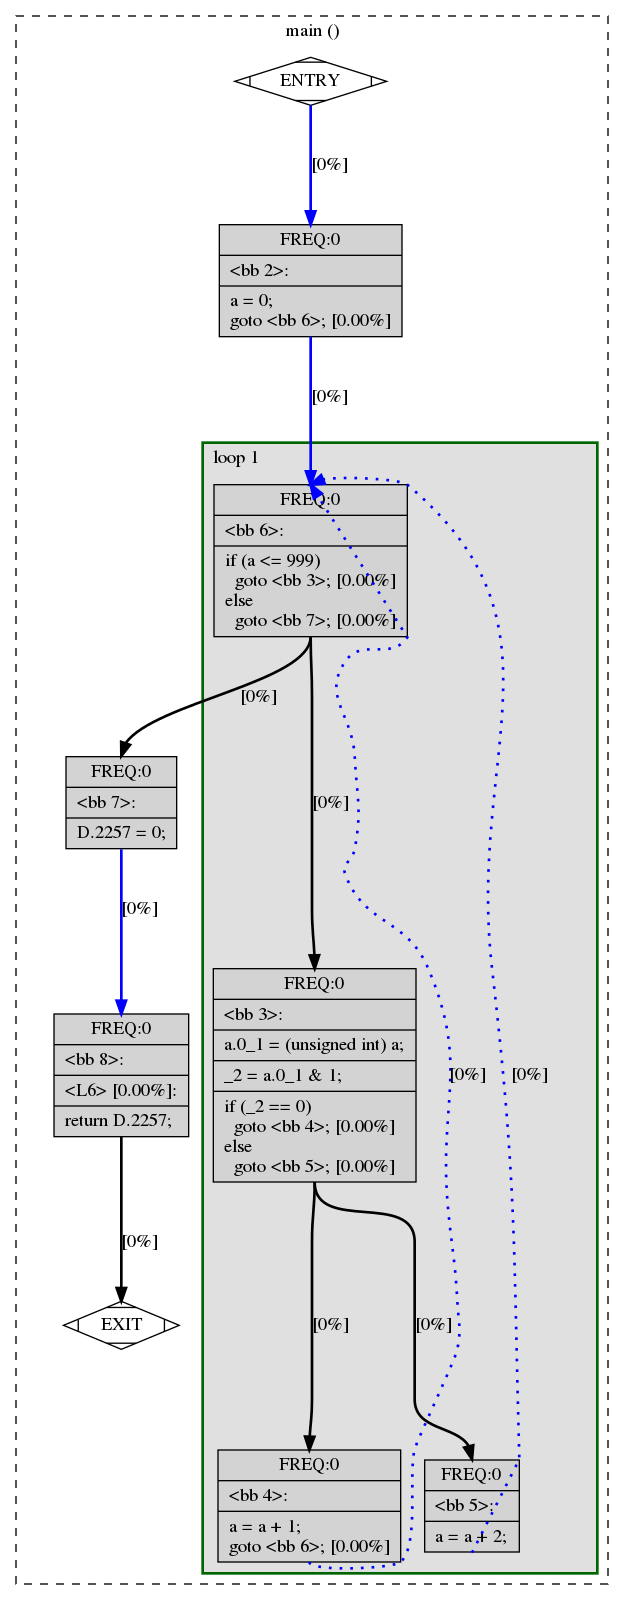
\includegraphics[scale=0.23]{graph.png}
    \captionof{figure}{Exemple CFG}
\end{center}
\end{multicols}
Comme l'exemple permet de le montrer, les graphes de flot de contrôle sont un excellent moyen de visualisation du code. Cependant sa véritable utilitée réside dans l'optimisation d'un code source.
\section{Nos recherches}

Afin d'étudier les Control Flow Graph, nous avons effectué un travail de recherche permettant de comprendre la modélisation des CFG, leur utilité et d'utiliser GCC pour générer et analyser des CFG. 

\subsection{Modélisation des CFG}
Nous allons dans un premier temps présenter la modélisation des CFG qui est déjà bien défini sur Wikipédia \cite{wiki:Graphe_de_flot_de_controle} mais approfondi dans la bible des compilateurs \cite{compilateurs}.

Les CFG font partis de la catégorie des graphes orientés. Cela signifie que ce sont des graphes dont les noeuds sont reliés par des arcs qui ont une direction. Les fonctions sont représentées par des sous-graphes disjoints les uns des autres.

Chaque noeud dans un CFG représente une portion de code, appelée \textbf{Bloc de base} dans laquelle il n'y a pas de saut ou de cible de saut. Un saut est défini par l'instruction \textit{goto xx} qui provient du langage assembleur et signifie \og saute à l'instruction xx \fg{}. L'entrée d'un bloc de base est la cible d'un saut, et la sortie est un saut.



Pour chaque fonction il existe toujours au moins deux blocs spéciaux. Le bloc \textit{Entry} qui caractérise l'entrée dans la fonction et donc le départ du flot, ainsi que le bloc \textit{Exit} qui caractérise la sortie de la fonction et la fin du flot.

Par construction le degré entrant et sortant d'un noeud, à part pour les blocs spéciaux définis ci-dessus, sont toujours supérieurs ou égaux à 1. En effet, si un bloc de base n'a pas de degré entrant, ce bloc n'est jamais exécuté et représente donc du code mort. Il peut alors être supprimé. De même, le seul bloc ayant un flot sortant nul est le bloc de sortie. 

Le code:
\begin{lstlisting}[numbers=left, xleftmargin=.35\textwidth]
    a = 0
    b = a + 70
    if b < 50
        print("Je ne vais pas afficher a")
        goto 7
    print(a)
    fin
\end{lstlisting}
se traduit en 4 blocs de base:
\begin{lstlisting}[xleftmargin=.35\textwidth]
    a = 0
    b = a + 70
    if b < 50

    print("Je ne vais pas afficher a")
    goto 7

    print(a)

    fin
\end{lstlisting}
et le graphe est représenté de la manière suivante:
\begin{center}
    \begin{tikzpicture}[
        node distance = 12mm and 6mm,
        box/.style = {rectangle, draw, fill=#1, 
                    minimum width=12mm, minimum height=7mm}
                    ]
        \node (n1) [box=white, align=justify] {a = 0\\b = a + 70\\if b < 50};
        \node (n2) [box=white, align=justify, below =of n1] {print("Je ne vais pas afficher a")\\goto 7};
        \node (n3) [box=white,below right=of n2] {print(a)};
        \node (n4) [box=white, below left=of n3] {fin};
        %
        \draw[->] (n1) to (n2);
        \draw[->, bend left] (n1) to (n3);
        \draw[->] (n2) to (n4);
        \draw[->] (n3) to (n4);

    \end{tikzpicture}
\end{center}
\section{Implémentation}
\subsection{Notre script de modifications des CFG}
\subsection{Notre analyse des CFG}